\documentclass[12pt]{article}
\usepackage{verbatim}
\usepackage[dvips]{epsfig}
\usepackage{color}
\usepackage{url}
\usepackage[colorlinks=true]{hyperref}

\begin{document}

\section*{GENESIS: Documentation}

\subsubsection*{Related Documentation:}
\href{../pub-purkinje-deschutter-morphology/pub-purkinje-deschutter-morphology.tex}{\bf Morphology}
% start: userdocs-tag-replace-items related-do-nothing
% end: userdocs-tag-replace-items related-do-nothing

\section*{De Schutter: Purkinje Cell Model}

\subsection*{Source}

De Schutter E \& Bower JM (1994) An active membrane model of the cerebellar Purkinje cell I. Simulation of current clamp in slice. {\it Journal of Nerurophysiology}. {\bf 71}: 375--400. \\

\subsection*{Figure}

\begin{figure}[h]
\centering
   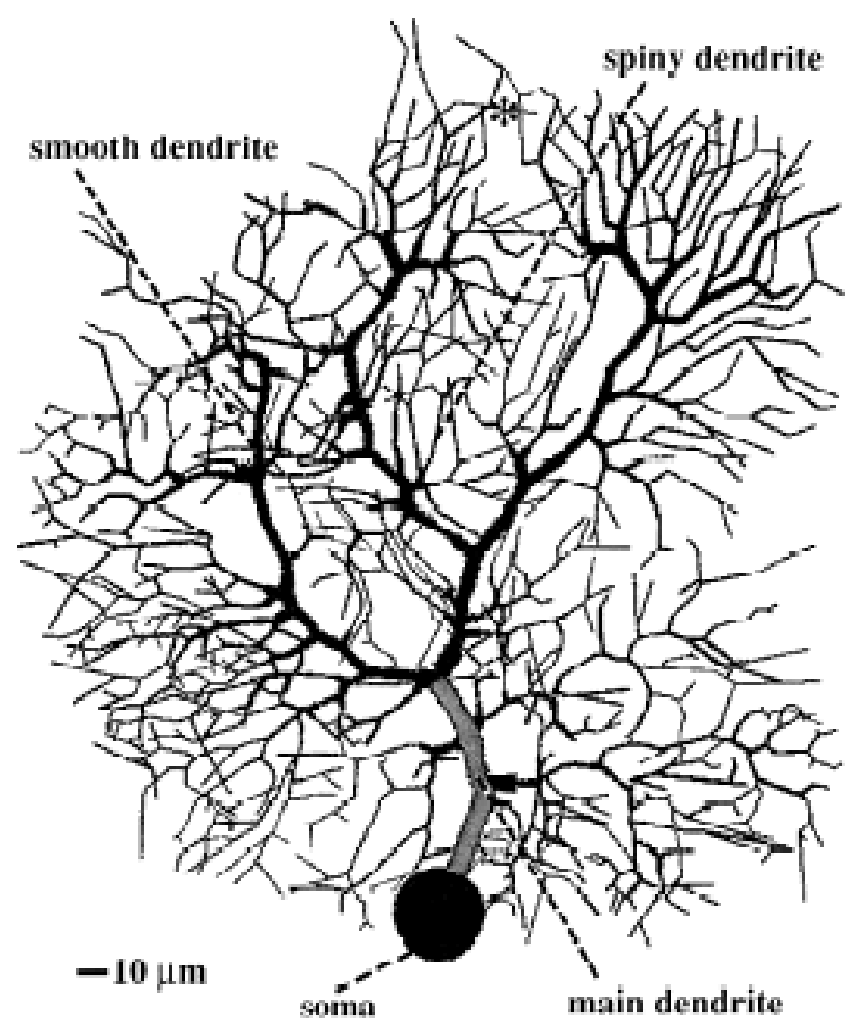
\includegraphics[scale=0.4]{figures/Fig.1.1.eps}
   \caption{Morphology of the Purkinje cell model ({\it cell\,1} of\,\cite{Rapp-P:1994qf}).  The 3 zones with different channel densities (Table 2) are marked
as soma (black), main dendrite (dark gray), and the rest of the dendrites
(black). Dashed lines: recording sites displayed in Figs 3-7. Asterisk: recording
site for Figs. 12 and 13.}
   \label{fig:DS1.1}
\end{figure}

\subsection*{Abstract}

A detailed compartmental model of a cerebellar Purkinje cell with active dendritic membrane was constructed. The model was based on anatomic reconstructions of single Purkinje cells.

\subsection*{Methods}

The morphology of the model was based on a detailed light microscopic reconstruction of horseradish peroxidase-filled guinea pig Purkinje cells by M. Rapp of the Hebrew University of Jerusalem, Israel\,\cite{Rapp-P:1994qf}.

\subsection*{Result}

\subsection*{Discussion}

\bibliographystyle{plain}
\bibliography{../tex/bib/g3-refs}

\end{document}
